Per riuscire a gestire in maniera adeguata il sempre maggior numero di device
connessi, e le diverse problematiche che essi comportano, è necessario andare a
cambiare le topologie di rete per fare in modo che rispecchino i punti necessari
per garantire il corretto funzionamento. Finora diversi standard sono stati
proposti, per risolvere queste problematiche. Ognuno di essi si basa sull'idea
del LPWAN \emph{Low power area network}. LPWAN è un termine usato per
identificare tutte quelle reti che permettono di connettere un numero elevato di
device in modo wireless per chilometri di distanza, riuscendo comunque a
mantenere basso il consumo energetico richiesto per la comunicazione. Inoltre
l'hardware utilizzato in questo tipo di rete ha un consto di produzione
relativamente basso , rendendole ottime per il mondo del IoT. Per raggiungere
questi punti, è necessario accettare dei compromessi sul numero di dati
trasmissibili e sulla banda utilizzata. 

\begin{figure}[h]
\centering 
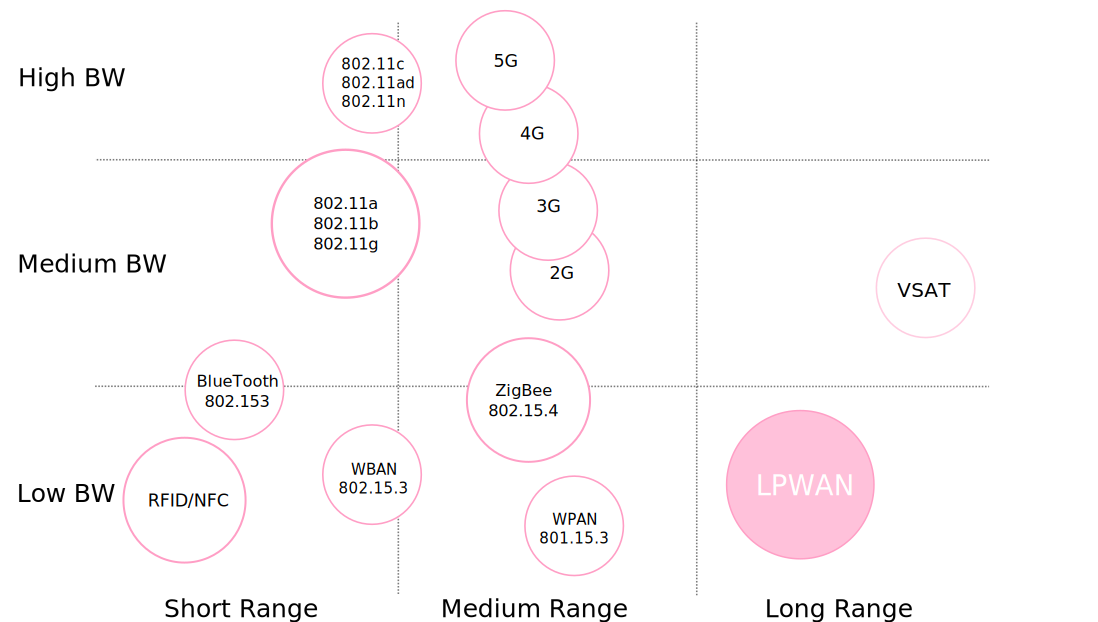
\includegraphics[width=16cm]{network_comp}
\caption{Comparazione tipologia di reti}
\end{figure}


